

%\begin{frame}
%    \frametitle{Свидетельство о регистрации программы}
%    \begin{figure}[h]
%        \centering
%        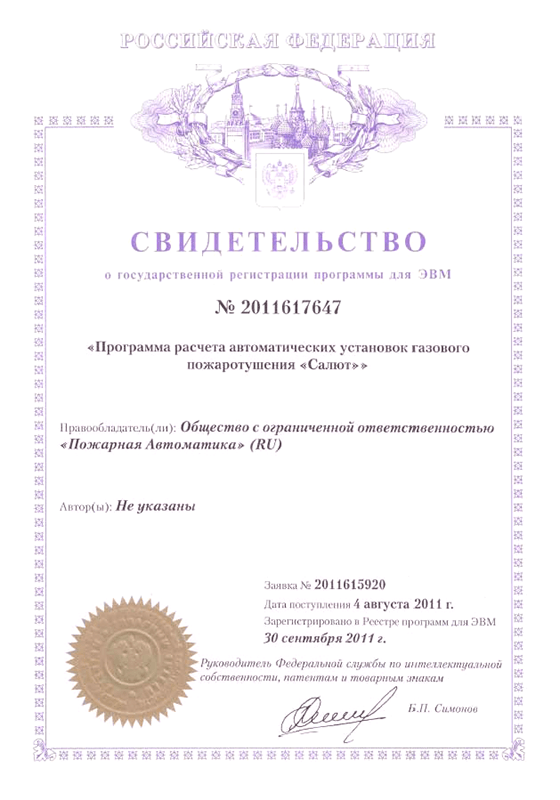
\includegraphics[height=0.7\textheight]{registration}
%    \end{figure}
%\end{frame}
%\note{
%    Получено свидетельство о регистрации разработанной программы \textsc{Hello~world™}.
%}

%\begin{frame}
%    \frametitle{Акт о внедрении}
%    \begin{figure}[h]
%        \centering
%        \fbox{
%            \begin{minipage}[t]{0.4\linewidth}
%                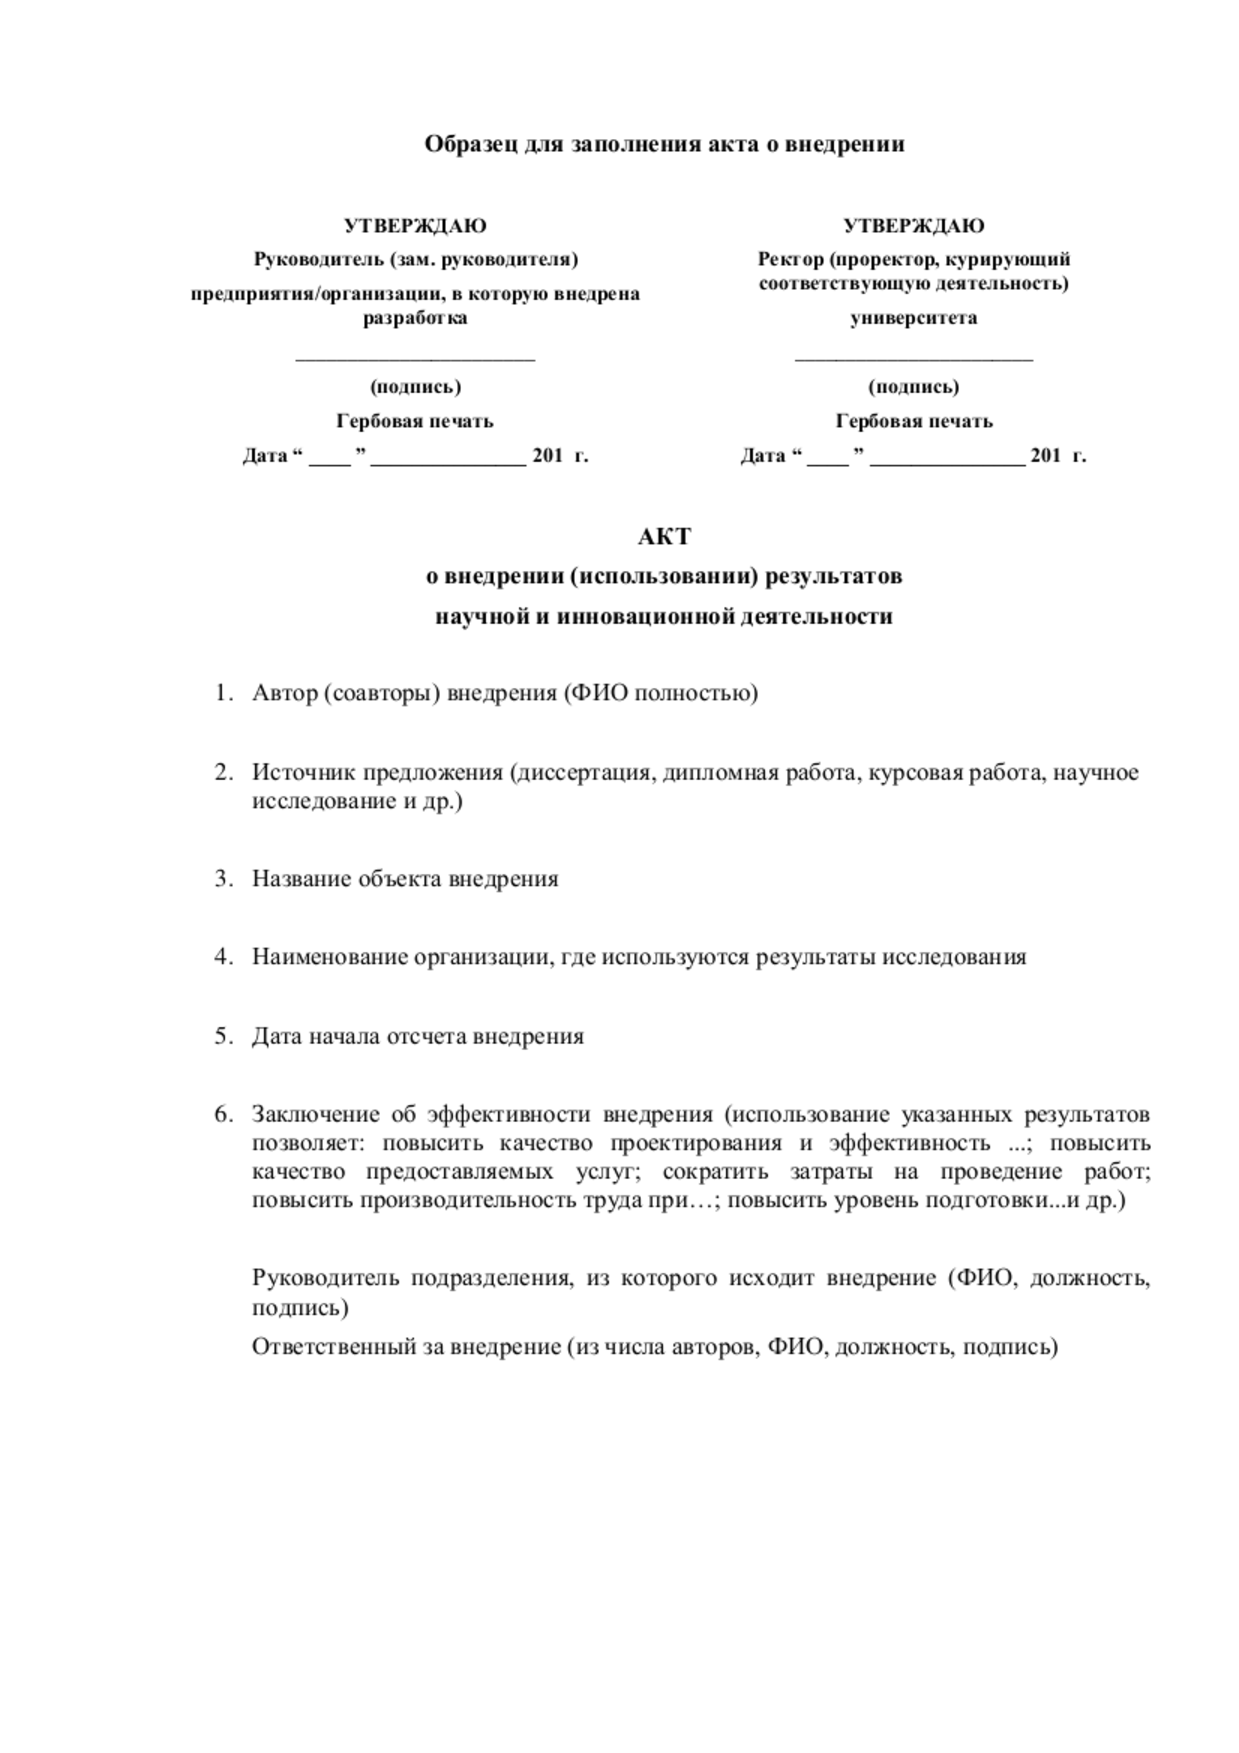
\includegraphics[width=\linewidth]{implementation}
%            \end{minipage}
%        }
%    \end{figure}
%\end{frame}
%\note{
%    Получен акт о внедрении.
%}


\begin{frame}
    \frametitle{Научная новизна}
    \begin{enumerate}
      \item Предложенный гибридный алгоритм дифференциальной эволюции отличается от известных ранее наличием процедуры адаптации штрафа.
      \item Учет инвариантности относительно равного сдвига фаз позволяет снизить размерность задачи и сократить среднее время счета решателя, основанного на методе ветвей и границ и локальном спуске.
      \item Впервые для задачи оптимизации направленности ФАР показано наличие кластеров из локальных оптимумов с одинаковым значением целевой функции, и не эквивалентных относительно равного сдвига фаз во всех излучателях.
      \item Впервые обоснована целесообразность учета взаимного влияния излучателей при оптимизации направленности ФАР КВ диапазона.
    \end{enumerate}
\end{frame}
\note{
Предложенный гибридный алгоритм дифференциальной эволюции отличается от известных ранее наличием процедуры адаптации штрафа, в которой учитывается возврат в допустимую область посредством масштабирования решения, что приводит к сокращению погрешности получаемых решений.
Ранее при решении задач оптимизации направленности ФАР, как правило, не использовалась инвариантность основных свойств решений относительно равного сдвига фаз во всех излучателях. Однако, как показано в настоящей работе, учет такой инвариантности позволяет снизить размерность задачи и сократить среднее время счета решателя, основанного на методе ветвей и границ и локальном спуске.
Впервые для задачи оптимизации направленности ФАР показано наличие кластеров из локальных оптимумов с одинаковым значением целевой функции, и не эквивалентных относительно равного сдвига фаз во всех излучателях.
Впервые обоснована целесообразность учета взаимного влияния излучателей при оптимизации направленности ФАР КВ диапазона.
}

\begin{frame}
    \frametitle{Практическая значимость}
    \begin{itemize}
      \item Разработанные алгоритмы оптимизации возбуждения ФАР могут применяться в системах связи коротковолнового диапазона для увеличения дальности радиосвязи.
      \item Созданное программное обеспечение позволяет производить необходимые для этого расчеты.
      \item Полученное обоснование необходимости учета взаимного влияния излучателей при оптимизации напраленности ФАР, а также, результаты вычислительных экспериментов для различных вариантов ФАР могут быть полезны при проектировании новых антенных систем.
    \end{itemize}
\end{frame}
\note{
Разработанные алгоритмы оптимизации возбуждения ФАР могут применяться в системах связи коротковолнового диапазона для увеличения дальности радиосвязи. Созданное программное обеспечение позволяет производить необходимые для этого расчеты. Полученное обоснование необходимости учета взаимного влияния излучателей при оптимизации напраленности ФАР, а также, результаты вычислительных экспериментов для различных вариантов ФАР могут быть полезны при проектировании новых антенных систем. Практическая значимость результатов исследования при выполнении работ по антенной тематике подтверждена в АО «Омский научно-исследовательский институт приборостроения».
}

\begin{frame}
    \frametitle{Теоретическая значимость}
    \begin{itemize}
      \item Осуществленный в работе переход от задачи оптимизации направленности ФАР в комплексных числах к задаче математического программирования позволил переформулировать в терминах математического программирования известные физические свойства задачи, в частности, инвариантность относительно сдвига фаз и закон сохранения энергии.
      \item Предложенная процедура возврата в допустимую область с помощью масштабирования вектора решения, а также построенная верхняя оценка эвклидовой нормы допустимых решений, могут быть использованы при разработке новых методов решения задач, аналогичных рассмотренной в работе.
    \end{itemize}
\end{frame}
\note{
Осуществленный в работе переход от задачи оптимизации направленности ФАР в комплексных числах к задаче математического программирования позволил переформулировать в терминах математического программирования известные физические свойства задачи, в частности, инвариантность относительно сдвига фаз и закон сохранения энергии. Предложенная процедура возврата в допустимую область с помощью масштабирования вектора решения, а также построенная верхняя оценка эвклидовой нормы допустимых решений, могут быть использованы при разработке новых методов решения задач, аналогичных рассмотренной в работе. Результаты диссертации используются в учебном процессе в ФГАОУ ВО «Омский государственный университет им. Ф.М. Достоевского» в составе лекционного курса «Эволюционные алгоритмы».
}


%\begin{frame}
%    \frametitle{Достоверность}
%    \textbf{Достоверность} научных положений, выводов и практических рекомендаций, полученных в диссертации, подтверждается точной формулировкой задач и критериев, достаточным количеством численных экспериментов и исследованиями адекватности модели с точки зрения физических принципов. Методика проведения численных экспериментов подробно описана, что позволяет воспроизвести полученные результаты.
%\end{frame}
%\note{
%Достоверность научных положений, выводов и практических рекомендаций, полученных в диссертации, подтверждается точной формулировкой задач
%и критериев, достаточным количеством численных экспериментов и исследованиями адекватности модели с точки зрения физических принципов. Методика проведения численных экспериментов подробно описана, что позволяет воспроизвести полученные результаты.
%}


\begin{frame}
    \frametitle{Апробация}
    \begin{itemize}
      \item Международная конференция <<Теория математической оптимизации и исследование операций (МОТОР)>> - Петрозаводск, июль, 2022; Иркутск, июль 2021; Екатеринбург, июль 2019.
      \item V Международной научно-технической конференции <<Радиотехника, электроника и связь>> - Омск, октябрь 2019.
      \item VII Международная конференции <<Проблемы оптимизации и их приложения>> - Омск, июль 2018.
      \item Семинар <<Математическое моделирование и дискретная оптимизация>>, ОФ ИМ СО РАН, Омск, 2018 — 2022.
      \item Семинар <<Современные проблемы радиофизики и радиотехники>>, ОмГУ им. Ф.М. Достоевского, Омск, 2021.
      \item Семинар <<Перспективы развития радиосвязи и приборостроения>>, АО <<ОНИИП>>, Омск, 2018.
    \end{itemize}
\end{frame}
\note{
Апробация работы. Основные результаты работы докладывались на конференциях: <<Теория математической оптимизации и исследование операций (МОТОР)>> в 2019, 2021 и 2022 годах, <<Радиотехника, электроника и связь>> - в 2019, <<Проблемы оптимизации и их приложения>> в 2018,
А также на семинарах <<Математическое моделирование и дискретная оптимизация>> с 2018 по 2022, <<Современные проблемы радиофизики и радиотехники>>, 2021, <<Перспективы развития радиосвязи и приборостроения>> в 2018.
}

%\begin{frame} % публикации на одной странице
 \begin{frame}[t,allowframebreaks] % публикации на нескольких страницах
    \frametitle{Основные публикации}
    \nocite{tyu:daor}%
    \nocite{tyu:jphys}%
    \nocite{tyu:motor}%
    \nocite{tyu:msim22}%
    \nocite{tyu22:ring}%
    \ifnumequal{\value{bibliosel}}{0}{
        \insertbiblioauthor
    }{
        \printbibliography%
    }
\end{frame}
\note{
    Основные результаты по теме диссертации изложены в 8 печатных изданиях, 4 из которых изданы в журналах, рекомендованных ВАК или прираненных к ним, 3 –– в тезисах докладов. Зарегистрирована 1 программа для ЭВМ.
}

\begin{frame}
    \frametitle{Основные результаты}
    \begin{enumerate}
 \item Задача оптимизации направленности ФАР имеет многочисленные локальные оптимумы, большое число из которых совпадают по целевой функции, однако не эквивалентны между собой с точностью до сдвига фаз.
  \item Учет фазовой симметрии позволяет снизить размерность задачи на одну переменную и сократить время счета коммерческого решателя BARON.
 \item Предложена модификация алгоритма дифференциальной эволюции в комбинации с градиентным алгоритмом, показавшая свою конкурентоспособность по сравнению с коммерческим решателем BARON.
  \item Обнаружено, что имеются конфигурации, при которых усиление ФАР существенно превосходит усиление одиночного излучателя, что может быть объяснено учетом взаимного влияния.
  \item Выявлены ситуации, в которых коэффициент усиления, соответствующий решению задачи квадратичной оптимизации, имеет существенное преимущество (до 5 дб) перед коэффициентом усиления, получаемым стандартным методом простого фазирования.
\end{enumerate}
\end{frame}

\begin{frame}[plain, noframenumbering] % последний слайд без оформления
    \begin{center}
        \Huge
        Спасибо за внимание!
    \end{center}
\end{frame}


\begin{frame}
    \frametitle{Основные положения, выносимые на защиту}
    \begin{enumerate}
      \item Задача имеет несколько кластеров из локальных оптимумов с одинаковым значением целевой функции, не эквивалентных относительно равного сдвига фаз во всех излучателях.
      \item Группа непрерывных симметрий рассматриваемой задачи одномерна и ее элементы соответствуют сдвигу фаз во всех излучателях на равную величину.
      \item Использование метода ДЭ в комбинации с градиентным подъемом позволяет достичь конкурентоспособных решений по сравнению с коммерческим решателем BARON в задаче оптимизации фаз и амплитуд ФАР.
      \item Имеется интервал параметров кольцевых ФАР, в котором учет взаимного влияния излучателей ведет к существенному увеличению коэффициента усиления в заданном направлении.
      \item Коэффициент усиления, соответствующий решению задачи оптимизации направленности ФАР, может быть существенно больше по сравнению с коэффициентом усиления, получаемым с помощью простого фазирования.
    \end{enumerate}
\end{frame}
\note{
Для большинства рассмотренных конфигураций ФАР задача имеет несколько кластеров из локальных оптимумов с одинаковым значением целевой функции, не эквивалентных относительно равного сдвига фаз во всех излучателях.

Группа непрерывных симметрий рассматриваемой задачи одномерна и ее элементы соответствуют сдвигу фаз во всех излучателях на равную величину, что позволяет снизить размерность задачи на одну переменную и сократить время счета.

Использование метода ДЭ в комбинации с градиентным подъемом позволяет достичь конкурентоспособных решений по сравнению с коммерческим решателем BARON в задаче оптимизации фаз и амплитуд ФАР, особенно на задачах большой размерности.

Имеется интервал параметров кольцевых ФАР, в котором учет взаимного влияния излучателей ведет к существенному увеличению коэффициента усиления в заданном направлении.

Коэффициент усиления, соответствующий решению задачи оптимизации направленности ФАР, может быть существенно больше по сравнению с коэффициентом усиления, получаемым стандартным методом фазирования без учета взаимного влияния (имеются случаи, когда отличие составляет 5 дб).

}

\begin{frame}
    \frametitle{Группы симметрий}
  Под линейной симметрией задачи будем понимать линейное преобразование P пространства поиска, имеющее вид~(\ref{eq:linsim}), заданное невырожденной матрицей $\textbf{P}$, такое что при подстановке новых координат y задача совпадает с исходной.% (т. е. все квадратичные формы от y оказываются теми же, что и исходные формы от $\textbf{x}$).
    \begin{equation}
    \textbf{x} \rightarrow \textbf{y} = \textbf{Px}
    \label{eq:linsim}
    \end{equation}
    \begin{equation}
    \textbf{H}_{\Sigma} = \sum_{j=1}^{M}\textbf{H}_j
    \end{equation}
    \begin{equation}
      \textbf{H}_{\Sigma} =\textbf{S}^T\textbf{DS}
    \end{equation}

    \vspace{1em}
    Далее считаем, что $\textbf{H}_{\Sigma}$ диагональна.

    \begin{equation}
    \label{eq:sunexp}
    \textbf{P}=e^{\sum\limits_n a_n G_n}=e^{\sum\limits_m a_m\hat{G}_m}
    \end{equation}

    \vspace{1em}

    \textbf{Еремеев А.В., Юрков А.С.:} On Symmetry Groups of Some Quadratic Programming Problems~// MOTOR 2020. Shpringer, 2020. Vol.~12095.
\end{frame}

\begin{frame}
    \frametitle{Группы симметрий}

    \begin{equation}
    \label{eq:commutat2}
    \left\{
    \begin{array}{l}
    \displaystyle
    {\bf H}_i \left(\sum\limits_na_nG_n\right) =
    \left(\sum\limits_na_nG_n\right){\bf H}_i \, , \\ \\
    \displaystyle
    {\bf G} \left(\sum\limits_na_nG_n\right) = \left(\sum\limits_na_nG_n\right){\bf G} \, .
    \end{array}
    \right.
    \end{equation}

    \vspace{3em}

    \textbf{Еремеев А.В., Юрков А.С.:} On Symmetry Groups of Some Quadratic Programming Problems~// MOTOR 2020. Shpringer, 2020. Vol.~12095.
\end{frame}

\begin{frame}
    \frametitle{Поиск группы непрерывных симметрий}
    \begin{itemize}
      \item Обработка. На этом этапе возможная неточность данных нивелируется усреднением симметричных компонент матриц (матрицы $\textbf{G}$ и $\textbf{H}$ должны быть симметричны).
      \item %Normalization of matrices $B_i$.
      Преобразование $ {\textbf{H}}_{\Sigma} = \sum_{i} \textbf{H}_i$ к канонической форме используя метод Лагранжа для вычисления матриц~$S$ и $S^{-1} $.
      \item Применение метода Гаусса к системе линейных уравнений~(\ref{eq:commutat2}) для вычисления генераторов~$\hat{G}_n$.
    \end{itemize}
\end{frame}
